\documentclass[11pt]{beamer}
\usetheme{CambridgeUS}
\usepackage[utf8]{inputenc}
\usepackage{amsmath}
\usepackage{amsfonts}
\usepackage{amssymb}
\usepackage{graphicx}

\author{Nico Fröhlich}
\title{Advanced CPU design and optimization}

\setbeamercovered{transparent} 
\setbeamertemplate{navigation symbols}{} 
\institute{Troblecodings} 
\subject{IT}

\begin{document}

\begin{frame}
    \titlepage
\end{frame}

\begin{frame}{Quellen und weiterführende Inhalte}
    \begin{itemize}
        \item Intel® 64 and IA-32 Architectures Software Developer’s Manual
        \item Software Optimization Guide for AMD64 Processors
        \item Intel® 64 and IA-32 Architectures Optimization Reference Manual
        \item Chandler Carruth, Matt Godbolt, Andrei Alexandrescu ...
        \item Mike Acton
        \item https://www.quick-bench.com/q/Ev6U1Owr7WKTbzyNgCol7vEJq4o
    \end{itemize}
\end{frame}

\begin{frame}{Einführung}
Das was alle CPUs gemeinsam haben:
    \begin{itemize}
        \item Clock (Oszillator)
        \item Fetch-Decode Cycle
        \item Instruction Counter
    \end{itemize}
\end{frame}

\begin{frame}{Fetch - Decode - Execute Cycle}
\begin{figure}[hbtp]
\centering
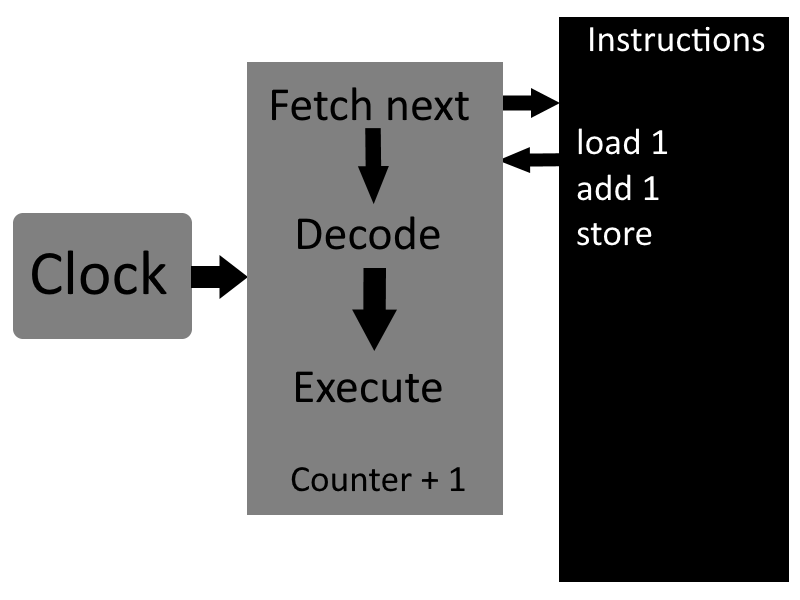
\includegraphics[scale=.4]{cpucycle.png}
\caption{CPU Cycle}
\end{figure}
\end{frame}

\begin{frame}
Let's talk cache
\begin{figure}[hbtp]
\centering
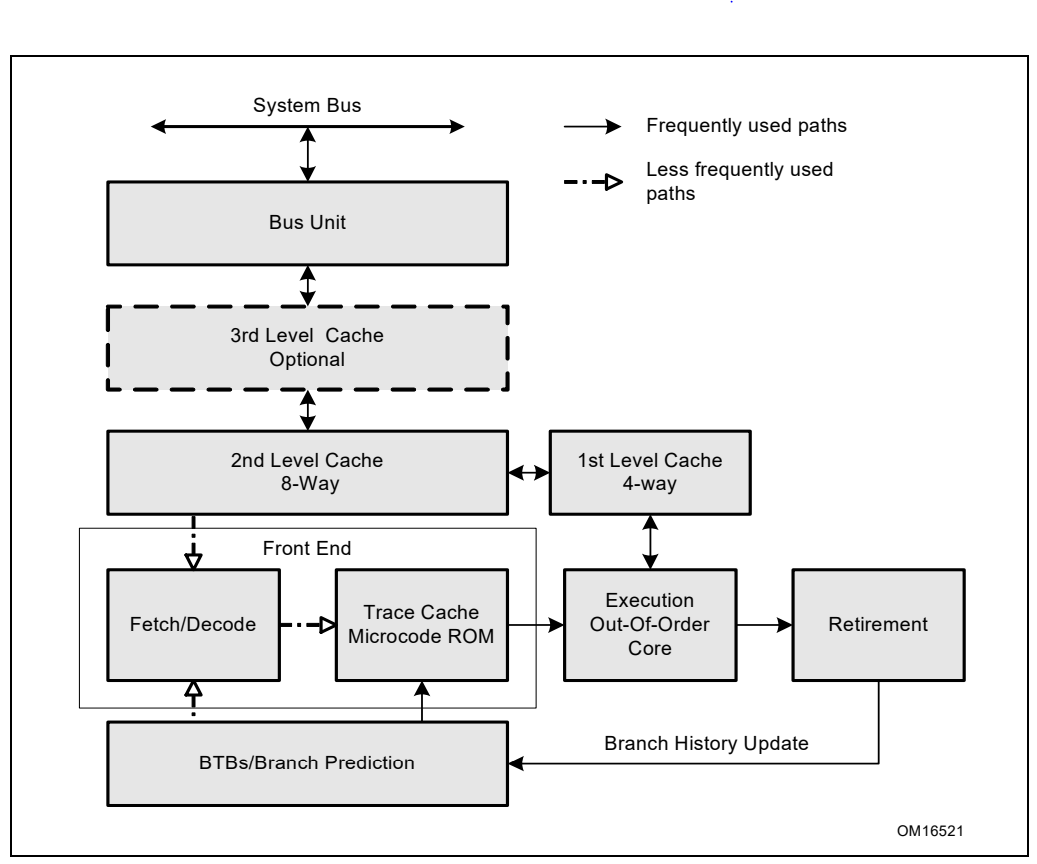
\includegraphics[scale=.3]{netburst.png}
\caption{The Intel NetBurst Microarchitecture}
\end{figure}
\end{frame}

\begin{frame}{Was passiert?}
\begin{itemize}
\item Die OOE zerlegt die gecacheten instructions
\item Schaut nach was für memory genutzt wurde
\item Fängt an die wahrscheinlichsten Sachen in den Cache zu laden
\item Executed was er kann
\item RU Updatet history und reordert instructions
\end{itemize}
\end{frame}

\begin{frame}{Cache misses}
\begin{figure}[hbtp]
\centering
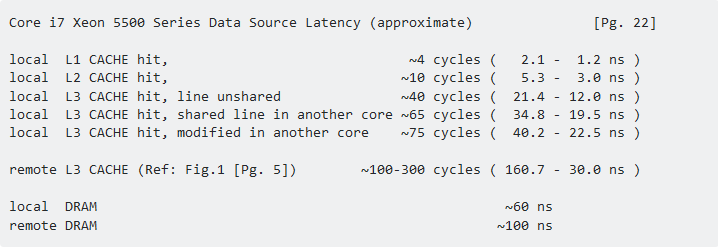
\includegraphics[scale=.5]{latency.png}
\caption{I7 Messungen}
\end{figure}
\end{frame}

\begin{frame}{Continues Memory ist gut}
\begin{columns}
\begin{column}{0.5\textwidth}

\begin{figure}[hbtp]
\centering
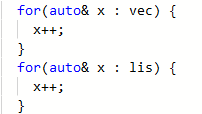
\includegraphics[scale=.6]{list.png}
\caption{Linked Lists}
\end{figure}

\end{column}
\begin{column}{0.5\textwidth}

\begin{figure}[hbtp]
\centering
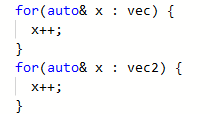
\includegraphics[scale=.6]{vec.png}
\caption{Continues memory}
\end{figure}

\end{column}
\end{columns}
\end{frame}

\begin{frame}{Ergebnisse}
\begin{figure}[hbtp]
\centering
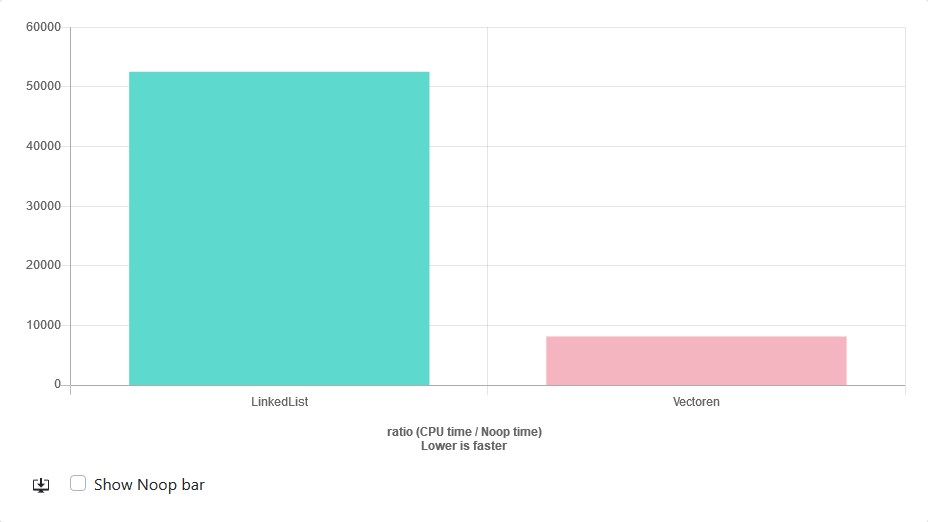
\includegraphics[scale=.35]{benchmark.png}
\caption{Quickbench ergebnisse}
\end{figure}
\end{frame}

\end{document}
